%%%%%%%%%%%%%%%%%%%%%%%%%%%%%%%
%%%%%%%%%%%%%%%%%%%%%%%%%%%%%%%
\chapter{Introduction}
%%%%%%%%%%%%%%%%%%%%%%%%%%%%%%%
%Section comments: Be mindful of using objective language. Avoid using general words like "good" or "special." It would also help to explain the example used for the Butterfly effect more.
The use of twin models is not a new idea. NASA built twin rockets for the Apollo missions, where one rocket went to the Moon and the other twin rocket stayed on Earth.
The twin model could have been used as a reference object in case of a mishap during the mission.  
The twin model concept has many other useful applications, not just for catastrophic scenarios with a failing space ship, but also for more ordinary applications for conventional ships. However, building a real twin ship as a reference object is not realistic. Instead, with data recorded aboard ships, it is possible to build a ship digital twin (SDT) to serve the same purpose.
System identification methods of rigid body ship dynamics are presented in this thesis, which can be used to build important sub-components/models in the SDTs. 

Ship dynamics is a branch of ship hydrodynamics that concerns the ship's forces and motions when the ship is allowed to move and rotate in all directions. Seakeeping and Manoeuvring are the two major subfields (see \autoref{fig:seakeeping_and_manoeuvring}). Seakeeping studies the  behavior of a ship in a seaway while it is under the influence of external waves, currents, and wind. Calm water conditions, lacking the external waves, are further assumed in Manoeuvring, which is considered either an idealized and simplified case of Seakeeping or the true conditions in sheltered environments. 
\begin{figure}
    \centering
    \begin{subfigure}[b]{0.45\textwidth}
         \centering
         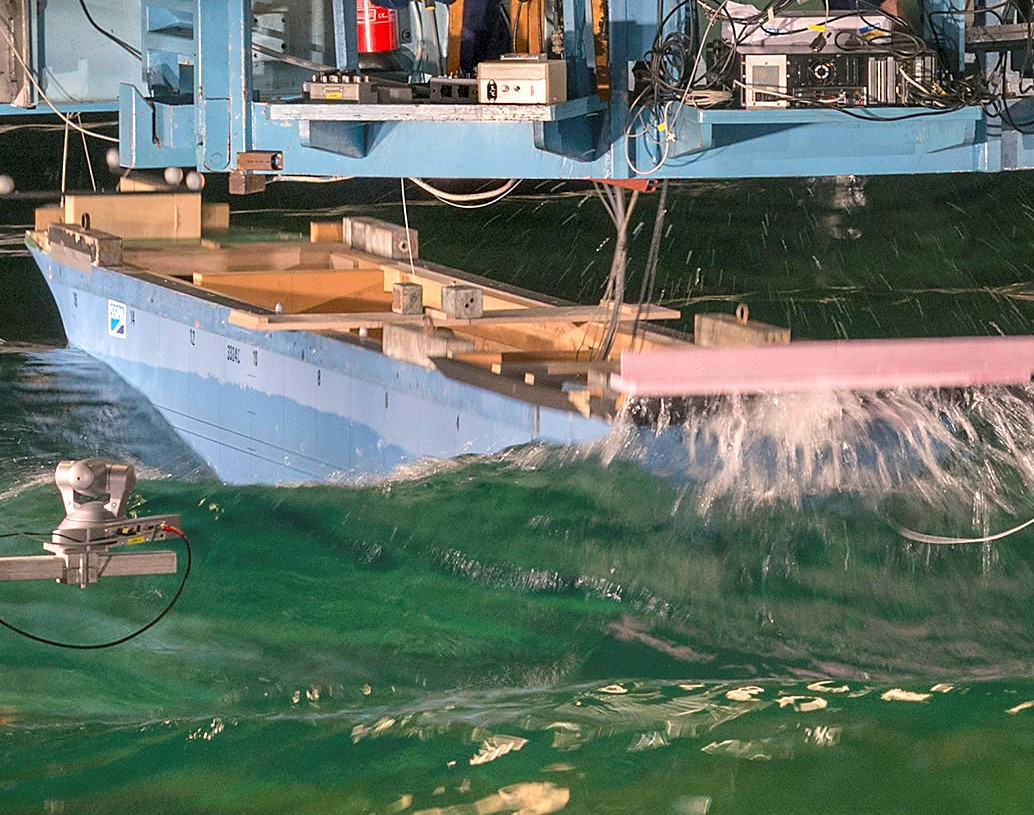
\includegraphics[width=\textwidth]{kappa/images/seakeeping.jpg}
         \caption{Seakeeping.}
         \label{fig:seakeeping}
     \end{subfigure}
     \hfill
     \begin{subfigure}[b]{0.45\textwidth}
         \centering
         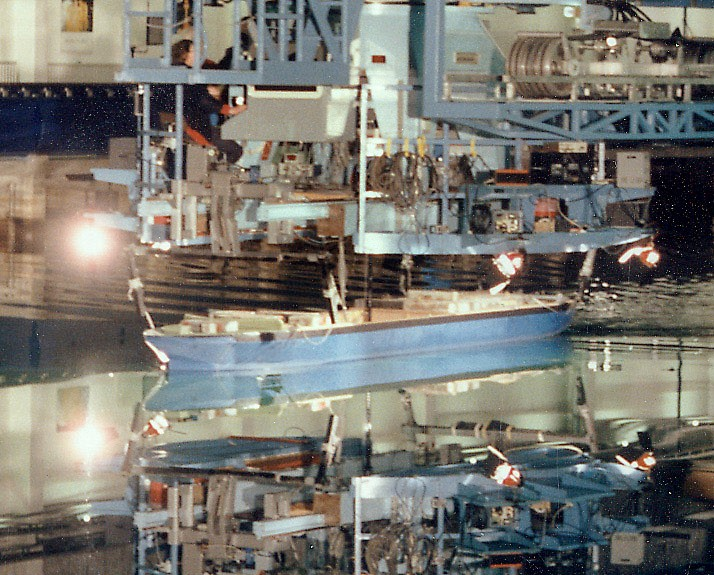
\includegraphics[width=\textwidth]{kappa/images/manoeuvring.jpg}
         \caption{Manoeuvring.}
         \label{fig:manoeuvring}
     \end{subfigure}
     \hfill
    \caption{Seakeeping and manoeuvring model tests, copyright SSPA.}
    \label{fig:seakeeping_and_manoeuvring}

\end{figure}
This chapter first provides a background by defining the Internet of Ships (IoS), ship digital twins (SDT) and the modelling of rigid body ship dynamics with white-box, black-box, or grey-box models. A literature review of system identification is then presented.
The motivation and objective of this research are then stated, followed by the assumptions and limitations.



\section{Background}
With the principles of the Industry 4.0, Shipbuilding 4.0 will transform the design, manufacturing, operation, shipping, services, production systems, maintenance, and value chains in all aspects of the shipbuilding 
industry \cite{stanic_toward_2018}.
The emergence of the Internet-of-Things (IoT) has led to the introduction of the Internet of Ships (IoS) paradigm. \begin{quote} IoS is the interconnecting of sensing objects, such as ships, crews, cargoes, onboard equipment, the waterway environment, waterway facilities, shore-based facilities, and other navigation elements. The sensing objects are embedded with various sensor and heterogeneous network technologies that enable them to collect and exchange data \cite{liu_internet_2016-1}.\end{quote}
Safety enhancements, route planning and optimization, energy efficiency, automatic berthing and autonomous shipping are some of the emerging applications of the IoS \cite{aslam_internet_2020}.
A ship digital twin (SDT), which is a digital copy of a real ship, is one way to utilize all data within the IoS \cite{chen_review_2021}. 
SDTs are data-driven in contrast to the alternative model-based virtual prototyping (VP) \cite{major_framework_2021}. An SDT is typically used as a model for an existing ship from which data can be collected; the VPs are  prototypes for future ships, in which no operational data is available.
The models for VP and SDT are categorized as white-box, black-box, or grey-box models.White-box models are used in VP. Either black-box or grey-box models are used in the SDTs. 
\begin{itemize}
    \item White-box modeling \\
    involves applying physical principles to ensure that no observed data is required. One example is computational fluid dynamics (CFD). Semi-empirical models, in which unknown physical constants have been derived from historical experiments, could also be considered white-box models \cite{leifsson_grey-box_2008}.  

    \item Black-box modeling \\
    means that parameters do not have physical significance and that the objective is to find an effective model that fits the observed data \cite{lindskog_tools_1995}.
    
    \item Grey-box modeling \\
    is using a combination of white-box and black-box modeling methods to ensure that both a physical model and data are used. This concept is also referred to as semi-physical modeling, hybrid modeling, or semi-mechanistic modeling in the literature \cite{leifsson_grey-box_2008}. 
\end{itemize}

\noindent The white and black component can be combined as a grey box model in several ways, using either a serial or parallel approach \cite{leifsson_grey-box_2008} as seen in Fig.\ref{fig:greycombinations}. 

\begin{figure}[H]
    \centering
    \begin{subfigure}[b]{0.3\textwidth}
    \centering
    \begin{tikzpicture}[node distance=2cm]
    \node (white-box) [white-box] {White-box};
    \node (black-box) [black-box, right of=white-box, xshift=2cm] {Black-box};
    \draw [arrow] (white-box) -- (black-box);
    \end{tikzpicture}
    \caption{Serial grey-box}
    \label{fig:serial1}
    \end{subfigure}

    
    \begin{subfigure}[b]{0.3\textwidth}
    \centering
    \begin{tikzpicture}[node distance=2cm]
    \node (black-box) [black-box] {Black-box};
    \node (white-box) [white-box, right of=black-box, xshift=2cm] {White-box};
    \draw [arrow] (black-box) -- (white-box);
    \end{tikzpicture}
    \caption{Serial grey-box}
    \label{fig:serial2}
    \end{subfigure}

    \begin{subfigure}[b]{0.3\textwidth}
    \centering
    \begin{tikzpicture}[node distance=2cm]
    \node (black-box) [black-box] {Black-box};
    \node (white-box) [white-box, below of=black-box] {White-box};
    \node (join) [process, right of=black-box, xshift=2cm, yshift=-1cm] {join};
    \draw [arrow] (black-box) -- (join);
    \draw [arrow] (white-box) -- (join);
    \end{tikzpicture}
    \caption{Parallel grey-box}
    \label{fig:parallel}
    \end{subfigure}
    \caption{Several ways to combine white- and black-box models in grey box models.}
    \label{fig:greycombinations}
\end{figure}

\section{Literature review}
Ship digital twin (SDT) has a positive trend in the number of publications in recent years (2018-2021)  \cite{assani_ships_2022}. Most of the papers concern ship equipment such as electric power systems, propulsion system, ship hull structure, and marine diesel engines \cite{assani_ships_2022}. A small minority of the SDT applications handle ship trajectory, speed, and fuel consumption \cite{assani_ships_2022}.   
Even though SDT is not explicitly mentioned, there are many publications about methods that can be used as SDTs. \textcite{lang_comparison_2022} predicted the propulsion power for a chemical tanker for three test case voyages by using ML black-box modeling. However, the manoeuvres were excluded. \textcite{nielsen_machine_2022} used grey-box modelling for the manoeuvring prediction of a ferry, where a deep learning model (black-box) captures the residues between a first-principles model (white-box) and observed data. These studies demonstrate the vast potential within the field.

Noteworthy publications within the system identification of the ship's manoeuvring dynamics are summarized in \autoref{tab:references} and categorized as black-box or grey-box models.
\begin{savenotes}\sphinxattablestart
\centering
\sphinxcapstartof{table}
\sphinxthecaptionisattop
\sphinxcaption{System identification references}\label{\detokenize{00.02_introduction:tab-methods}}
\sphinxaftertopcaption
\begin{tabulary}{\linewidth}[t]{|T|T|T|T|T|}
\hline
\sphinxstyletheadfamily 
\sphinxAtStartPar
Method
&\sphinxstyletheadfamily 
\sphinxAtStartPar
BB
&\sphinxstyletheadfamily 
\sphinxAtStartPar
GB
&\sphinxstyletheadfamily 
\sphinxAtStartPar
Data
&\sphinxstyletheadfamily 
\sphinxAtStartPar
Reference
\\
\hline
\sphinxAtStartPar
Constrained Least Squares
&
\sphinxAtStartPar
x
&&
\sphinxAtStartPar
model test, CFD
&
\sphinxAtStartPar
\cite{araki_estimating_2012}
\\
\hline
\sphinxAtStartPar
Neural network
&
\sphinxAtStartPar
x
&&
\sphinxAtStartPar
model test
&
\sphinxAtStartPar
\cite{he_nonparametric_2022}
\\
\hline
\sphinxAtStartPar
Gaussian process
&
\sphinxAtStartPar
x
&&
\sphinxAtStartPar
model test
&
\sphinxAtStartPar
\cite{xue_identification_2021}
\\
\hline
\sphinxAtStartPar
Kalman filter maximum likelihood
&&
\sphinxAtStartPar
x
&
\sphinxAtStartPar
full scale
&
\sphinxAtStartPar
\cite{astrom_identification_1976}
\\
\hline
\sphinxAtStartPar
Unscented kalman filter
&&
\sphinxAtStartPar
x
&
\sphinxAtStartPar
full scale
&
\sphinxAtStartPar
\cite{revestido_herrero_two-step_2012}
\\
\hline
\sphinxAtStartPar
Extended kalman filter
&&
\sphinxAtStartPar
x
&
\sphinxAtStartPar
full scale
&
\sphinxAtStartPar
\cite{perera_system_2015}
\\
\hline
\sphinxAtStartPar
Extended kalman filter
&&
\sphinxAtStartPar
x
&
\sphinxAtStartPar
simulated
&
\sphinxAtStartPar
\cite{shi_identification_2009}
\\
\hline
\sphinxAtStartPar
SVR
&&
\sphinxAtStartPar
x
&
\sphinxAtStartPar
simulated
&
\sphinxAtStartPar
\cite{zhu_parameter_2017}, \cite{wang_parameter_2021}
\\
\hline
\sphinxAtStartPar
SVR
&&
\sphinxAtStartPar
x
&
\sphinxAtStartPar
model test
&
\sphinxAtStartPar
\cite{luo_parameter_2016}
\\
\hline
\sphinxAtStartPar
Genetic algorithm
&&
\sphinxAtStartPar
x
&
\sphinxAtStartPar
lake test
&
\sphinxAtStartPar
\cite{miller_ship_2021}
\\
\hline
\end{tabulary}
\par
\sphinxattableend\end{savenotes} 
\noindent The system identification can be applied to full scale data \cite{astrom_identification_1976,revestido_herrero_two-step_2012,perera_system_2015}, which has the highest model uncertainty and measurement uncertainty. Therefore, it is the hardest task but also the most relevant. A method for reducing the uncertainty is using model test data, as in \cite{araki_estimating_2012,luo_parameter_2016,xue_identification_2021,miller_ship_2021, he_nonparametric_2022}. The uncertainty can be further reduced by using simulated data, as in \cite{shi_identification_2009,zhu_parameter_2017,wang_parameter_2021}, which can demonstrate the potential of new methods that have the benefit of the true model being known. One must however be consistent with the main objective of identifying real objects, not only mathematical models \cite{miller_ship_2021}.

\noindent Black-box modeling was used in \textcite{he_nonparametric_2022}, using a neural network, and in \textcite{xue_identification_2021}, using a Gaussian process. The nonparametric models are related because the system structure is known but no parameters are required; this is seen in \textcite{pongduang_nonparametric_2020}. However, most of the system identification methods for ship manoeuvring models use grey-box modeling by assuming a predefined mathematical model, which reduces the problem to a parameter estimation.
The Kalman filter (KF) combined with maximum likelihood estimation was proposed in 1976 by \textcite{astrom_identification_1976} to develop a linear manoeuvring model that utilized manually recorded data in 1969 aboard the Atlantic Song freighter. The extended Kalman filter (EKF) can also estimate parameters if the parameters are represented as states of the state space model. This technique was used on a nonlinear Nomoto model \cite{perera_system_2015} and a 3 degree of freedom model (3DOF) \cite{shi_identification_2009}. The EKF was used in \textcite{araki_estimating_2012}, with constrained parameters based on physical reasoning and prior knowledge from constrained least squares regression. The unscented Kalman filter (UKF), which has been proposed as an improvement to the EKF for handling nonlinear systems, was used in \textcite{revestido_herrero_two-step_2012}.
Support vector regression (SVR) has been investigated in \cite{luo_parameter_2016,zhu_parameter_2017, wang_parameter_2021}. A genetic algorithm was used by \textcite{miller_ship_2021} for the system identification of a model test performed on a lake.





%"Critic" to what has been done before
\section{Motivation and objective}
\label{sec:motivation}
% Motivation:
A profuse amount of data concerning the operation of ships in the oceans is collected daily. Many uses and potential applications of this data remains to be discovered. The use of SDTs (which are modelled as white-boxes, black-boxes, or grey-boxes) has potential .
Black-box modeling is entirely data-driven, which means that no prior understanding of the system generating the data is needed. Therefore, it is an attractive option for the SDT modelling. One caveat is that the black-box modeling may provide infeasible models outside of the domain covered by the available data \cite{nielsen_machine_2022}. 

The white-box modeling, which is not relying on the data, does not have this problem. However, to obtain high accuracy it does require a complete understanding of the system. Acquiring such knowledge may be possible for some cases with CFD calculations, but it is not practical for the complex environment and nonlinearities of a ship operating at sea \cite{miller_ship_2021}. 
Wind, waves, and currents add uncertainty to the modelling in the deep sea. Water depth and the bank effect add uncertainty in coastal areas \cite{nielsen_machine_2022}. 
Even if the sea is flawlessly modelled, long-term predictions with high accuracy will be exposed to deterministic chaos \cite{lorenz_deterministic_1963}, which is popularly known as the butterfly effect. During the butterfly effect, only a very small difference in the initial conditions results in a significantly different outcome. For instance, a period of two weeks is believed to be the upper limit for weather forecasts  \cite{zhang_what_2019}. Because the methods developed in this thesis frame the first step towards system identification in full scale sea conditions, grey-box modelling is used. The grey-box model involves merging the white-box and black-box methods in an attempt to alleviate concerns regarding both models. 

It is practical to first assume higher levels of simplifications and approximations for the problem under study and thereafter increase the complexity of the problem step by step. The effects of various factors can be initially studied in isolation with this approach. 
rigid body ship dynamics at full scale sea conditions comprises uncertainties from:
\begin{itemize}
    \item the \textbf{environment}: wind, waves, and currents
    \item the \textbf{ship}: geometry and mass properties
    \item the \textbf{measurements}
\end{itemize}

\noindent The simplification this thesis presents is limiting the uncertainties at full scale sea conditions by using model test data from a controlled laboratory environment. The main objective of this thesis is to:
% Objective: 
\begin{quote} 
\expandafter\MakeUppercase \objective
\end{quote}

\noindent 
To fulfill the research objective, the goals for this thesis have been formulated by following the step-by-step approach. The approach consists of reducing complexity and then gradually increasing the model complexity:

\subsubsection*{\normalfont \color{black} \textbf{Roll motion model}}
The first goal of the thesis is to develop a model for the calm water rigid body ship dynamics in the roll degree of freedom; it is based on model test data.

\subsubsection*{\normalfont \color{black} \textbf{Manoeuvring model}}
The second goal is to increase the complexity and uncertainty of the modelling by adding the surge, sway, and yaw degrees of freedom, which addresses the manoeuvring problem.

\subsubsection*{\normalfont \color{black} \textbf{Model generalization}}
The third goal is a constraint. In order to be of practical use in the internet of ships (IoS) applications, the models must be able to make predictions outside of the domain covered by the available data.

\section{Assumptions and limitations}
%Calm waters...
The calm water condition is used as a simplification of the real sea condition that a ship encounters. This condition does not account for the factors of wind, waves, and currents. These assumptions simplify the system identification by reducing the degrees of freedom to: surge, sway, yaw and, roll. 
The rigid body assumption simplifies the ship to a stiff body that does not transform under the influence of forces. 
It is important to note that all results are not necessarily directly transferable to the full scale when model scale data is used considering potential scale effects. 

\section{Reproducibility}
The research for this thesis has been conducted with the aim of having a high degree of reproducibility. The U.S. National Science Foundation (NSF) subcommittee on replicability in science defines reproducibility as:
\begin{quote}
Reproducibility refers to the ability of a researcher to duplicate the results of a prior study
using the same materials and procedures as were used by the original
investigator. 
E.g., a researcher uses the same raw data, builds same analysis files,
and same statistical procedures to make sure that same results
obtained as in published study. Reproducibility is a minimum necessary condition for a finding to be
believable and informative. 
    \cite{bollen_reproducibility_2015}
\end{quote}

\noindent To ensure adequate reproducibility, all code developed in this research has been made available as open source. In addition, the used data has been published as open data, as seen in the references in \autoref{tab:reproducibility}. Publishing the roll decay data from Paper \ref{pap:rolldamping} as open data was not possible due to intellectual property (IP) rights.

\begin{table}[H]
    \centering
    \caption{References for reproducibility.}
    \label{tab:reproducibility}
    \begin{tabular}{ c l l}
        \toprule
         Paper &  Code & Data \\
         \hline
         \ref{pap:rolldamping} & \textcite{alexandersson_rolldecay-estimators_2022} & Unpublished due to IP rights\\
         \ref{pap:pit} & \textcite{alexandersson_code_2022} & \textcite{alexandersson_wpcc_2022}, \textcite{stern_experience_2011} \\
         \bottomrule
    \end{tabular}
\end{table}

\section{Outline of the thesis}
Chapter \ref{ch:models} presents the models for rigid body ship dynamics used in this thesis. The models for roll motion are introduced in \autoref{sec:roll}, and the manoeuvring motion models are introduced in  \autoref{sec:manoeuvring model}. These models represent the physical principles and thereby the white-box component of the developed grey-box models.
Parameter estimations, representing the black-box component, are used to regress the parameters of the white-box models. The parameter estimations are introduced in \autoref{ch:methods} for the roll motion and the manoeuvring motion in \autoref{sec:_roll} and \autoref{sec:_VMM}. 
A summary of the appended papers, which includes research activities and a selection of the most relevant results, is presented in \autoref{ch:results}, followed by the conclusions in \autoref{ch:conclusions} and plans for future work in \autoref{ch:future_work}.